\documentclass[tikz,border=8pt]{standalone}
\usepackage{amsmath}
\usetikzlibrary{arrows.meta,positioning,fit}

\begin{document}
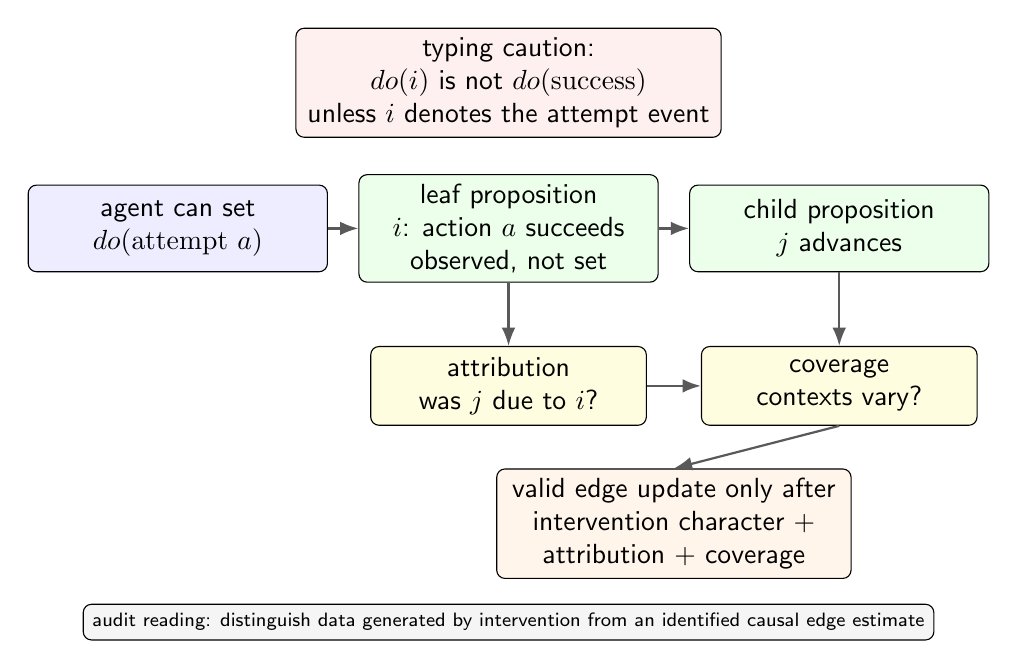
\begin{tikzpicture}[
  font=\sffamily,
  box/.style={draw, rounded corners=3pt, align=center, minimum width=38mm, minimum height=11mm, fill=white},
  gate/.style={draw, rounded corners=3pt, align=center, minimum width=35mm, minimum height=10mm, fill=yellow!12},
  note/.style={align=center, font=\sffamily\scriptsize},
  arrow/.style={-Latex, thick, draw=black!65},
  warn/.style={-Latex, thick, dashed, draw=orange!85!black}
]

\node[box, fill=blue!7] (attempt) at (0,0)
  {agent can set\\$do(\mathrm{attempt}\ a)$};
\node[box, fill=green!8] (success) at (4.2,0)
  {leaf proposition\\$i$: action $a$ succeeds\\observed, not set};
\node[box, fill=green!8] (child) at (8.4,0)
  {child proposition\\$j$ advances};

\draw[arrow] (attempt) -- (success);
\draw[arrow] (success) -- (child);

\node[gate] (attr) at (4.2,-2)
  {attribution\\was $j$ due to $i$?};
\node[gate] (ctx) at (8.4,-2)
  {coverage\\contexts vary?};
\draw[arrow] (success.south) -- (attr.north);
\draw[arrow] (child.south) -- (ctx.north);
\draw[arrow] (attr.east) -- (ctx.west);

\node[box, fill=orange!8, minimum width=45mm] (valid) at (6.3,-3.75)
  {valid edge update only after\\intervention character +\\attribution + coverage};
\draw[arrow] (ctx.south) -- (valid.north);

\node[box, fill=red!6, minimum width=54mm] at (4.2,1.85)
  {typing caution:\\$do(i)$ is not $do(\mathrm{success})$\\unless $i$ denotes the attempt event};

\node[note, fill=gray!8, draw, rounded corners=3pt, minimum width=88mm] at (4.2,-5.0)
  {audit reading: distinguish data generated by intervention from an identified causal edge estimate};

\end{tikzpicture}
\end{document}
